\documentclass[onecolumn, draftclsnofoot,10pt, compsoc]{IEEEtran}
\usepackage{graphicx}
\usepackage{url}
\usepackage{setspace}
\usepackage[font=small,labelfont=bf]{caption} % Required for specifying captions to tables and figures
\usepackage{geometry}
\geometry{textheight=9.5in, textwidth=7in}

% 1. Fill in these details
\def \CapstoneTeamName{		Malsano}
\def \CapstoneTeamNumber{		72}
\def \GroupMemberOne{			Katherine Jeffrey}
\def \GroupMemberTwo{			Brandon Jolly}
\def \GroupMemberThree{			Bradford Wong}
\def \CapstoneProjectName{		App to Support Field Diagnostics in Veterinary Medicine}
\def \CapstoneSponsorCompany{	Oregon Veterinary Diagnostics Laboratory}
\def \CapstoneSponsorPerson{		Professor Christiane Loehr}

% 2. Uncomment the appropriate line below so that the document type works
\def \DocType{		%Problem Statement
				%Requirements Document
				%Technology Review
				%Design Document
				Progress Report
				}
			
\newcommand{\NameSigPair}[1]{\par
\makebox[2.75in][r]{#1} \hfil 	\makebox[3.25in]{\makebox[2.25in]{\hrulefill} \hfill		\makebox[.75in]{\hrulefill}}
\par\vspace{-12pt} \textit{\tiny\noindent
\makebox[2.75in]{} \hfil		\makebox[3.25in]{\makebox[2.25in][r]{Signature} \hfill	\makebox[.75in][r]{Date}}}}
% 3. If the document is not to be signed, uncomment the RENEWcommand below
\renewcommand{\NameSigPair}[1]{#1}

%%%%%%%%%%%%%%%%%%%%%%%%%%%%%%%%%%%%%%%
\begin{document}
\begin{titlepage}
    \pagenumbering{gobble}
    \begin{singlespace}
    	
\includegraphics[height=4cm]{coe_v_spot1}
        \hfill 
        % 4. If you have a logo, use this includegraphics command to put it on the coversheet.
        %\includegraphics[height=4cm]{CompanyLogo}   
        \par\vspace{.2in}
        \centering
        \scshape{
            \huge CS Capstone \DocType \par
            {\large\today}\par
            \vspace{.5in}
            \textbf{\Huge\CapstoneProjectName}\par
            \vfill
            {\large Prepared for}\par
            \Huge \CapstoneSponsorCompany\par
            \vspace{5pt}
            {\Large\NameSigPair{\CapstoneSponsorPerson}\par}
            {\large Prepared by }\par
            Group\CapstoneTeamNumber\par
            % 5. comment out the line below this one if you do not wish to name your team
            \CapstoneTeamName\par 
            \vspace{5pt}
            {\Large
                \NameSigPair{\GroupMemberOne}\par
                \NameSigPair{\GroupMemberTwo}\par
                \NameSigPair{\GroupMemberThree}\par
            }
            \vspace{20pt}
        }
        \begin{abstract}
        % 6. Fill in your abstract    
        	Currently, there are many difficulties for veterinary pathologists trying to perform remote diagnostics. There are not any effective ways for people out in the field collecting samples to communicate with specialized experts located in laboratories. As a result, this project will involve creating an android mobile application that will be used as a bridge to connect the field personnel with the veterinary pathologists in laboratories. With this mobile application, the field personnel will be able to take pictures of the individual that is being analyzed and then send the pictures along with other data such as the patient, location, and time to a pathologist. The pathologist will then be able to use the provided information to perform a necropsy and send feedback to the field personnel. This project is intended to support remote field diagnostics in veterinary medicine.
        \end{abstract}     
    \end{singlespace}
\end{titlepage}
\newpage
\pagenumbering{arabic}
\tableofcontents
% 7. uncomment this (if applicable). Consider adding a page break.
%\listoffigures
%\listoftables
\clearpage

% 8. now you write!
\section{Project Purpose and Goals}
The completed project components are intended to serve as a means of communication between personnel in the field and pathologists in the laboratory. It's purpose is to improve a team's ability to perform remote diagnostics by providing a convenient way for teams to communicate information. The OVDL wants a native Android mobile application that collects field data and images, stores the information on a native SQLite database, sends them to the lab’s MySQL database, and gets real time feedback from the lab. The lab will interact with the database and user's submissions through the website.

\section{Progress and Plans}
\subsection{Completed Parts of Project}
\subsubsection{Database}
Figure 1 displays the code used to create a Submission table in the Mysql database. Currently we are only creating a small version of the Submission table for testing purposes. Once we have determined we can reliably send information from the SqLite database to the server where Mysql is located then we would begin the process of fully flushing out the database on the server end. Figure 2 displays the current SqLite Database in android. This database is more flushed out in order to test portions of the android app. Like the MySql database, the tables are currently in testing form and as such do not have the all the necessary functions needed for each table. As an example we do not have a Accessor for the column Submitted. Though we do have them for the internalID, Title, and Date Of Creation. 

\subsubsection{Android}
The team has made significant progress on the Android application. The home screen has been completely implemented. All of the navigation buttons have been added and they all take the user to the corresponding screens. Additionally, the toolbar has been implemented and can take the user to any of the relevant screens.

Clicking on the "Create Account" button successfully opens up a web browser. For now, it just takes the user to the Oregon Veterinary Diagnostic Laboratory's website.

For the create submissions screen, all of the input fields were added. The "Save Draft" and "Submit" buttons correctly store some of the submission data into the SQLite database. Additionally, the "Add Pictures" screen has been implemented. Users can upload five pictures using either the camera or the phone's gallery and can also delete the pictures they uploaded. Also, the application can track all of the meta data of the pictures, including the name of the picture, the date it was taken, and the GPS coordinates. 

For the "View Drafts" screen, all of the drafts stored in the database can be seen in a list. Additionally, users can remove drafts from the database by long clicking on the entry in the list.

For the "View Submissions" screen, the user can view all of the submissions that they submitted to the database in a list. The user can also click on an entry and the app will successfully navigate to that submission's detailed page. Like the View Drafts screen, the user can delete submissions from the database by long clicking on the submission in the list. Each entry in the list also shows the relevant information such as the submission title, the case ID, and when the submission was created.

\subsubsection{Website}
All the pages of the website have been created with basic layouts and some input validation for the login and registration pages. The pages ensure input fields are filled properly before submitting to the database for processing. The main page is the submissions page that has a table of all the submissions available to the user. The table shows the submission title, the name of the user that submitted it, its case ID and the date it was received. When clicked the individual submissions open a case detail page with the rest of the submission data. This is where messages will be processed. Users will be able to send messages about the submission to the submitter's phone. 

There is also an account page where users can change their username or password. An about page is also included to provide users with information about the site, the app, and how to use them or contact people who can assist them. The pages are all accessible to each other though a navigation bar at the top of the pages. The website is currently hosted on an OSU server, but it will be moved to the client's server when it is ready. 


\subsection{Parts of Project Left to Complete}
\subsubsection{Database}
Both databases need to be fully created. Figure 3 is a diagram of the tables needed to be implemented for each database. and a key which explains the colors associated with the table. In addition to the tables needing to be added to the respective database. Functions for the SqLite tables also need to be implemented in the android app. This functions include: Accessors, Modifiers, and any unique functions associated with the table. 
\subsubsection{Android}
The team still needs to fully complete all work that uses the API. The client is still developing the API, so the team hasn't been able to work on any tasks that involve it. This includes handling login and logout, sending 
data from the phone to the server, and receiving comments on submissions from the website. Additionally, clicking on the "Create Account currently opens up the OVDL's website. The team will need to change the URL that the app opens up once the website has been hosted. The team also still needs to store the rest of the submission data into the SQLite database and have that data be stored on the detail submission page. The drafts functionality still needs to be implemented because clicking on a draft doesn't navigate the user to a new screen with the fields filled out already. Lastly, the team needs to implement the settings and isntructions screens.
\subsubsection{Website}
The website still needs to be transferred to the client's Ubuntu server. There is still work being done on the server so the web pages are being designed separately. The website has also not been connected to the database for a similar reason. The MySQL database is still being completed as well as the API that will facilitate their communication. Once those pieces are ready to connect some choices about the login and registration process will need to be made. The clients will need to decide how much security is necessary and specify the differences between user groups. We have discussed having levels of privileges for general users, OVDL affiliated users, and OVDL veterinary pathologist users. It is still unclear how security levels will be assigned and enforced. 

Another important piece that is sill unclear is messaging. We know pathologists will need to send messages to users about their submissions, but it is unclear if pathologists will also send messages to each other or how security levels will affect the messaging system. Unstable network connectivity is also a concern so we will need to implement a way of handling potential internet interruptions. 

\section{Problems}
The first issue we had was one of our team members was unable to push anything to our android repository. He was able to pull information but when he tried to push it would say he did not have authorization. We checked the repository to see if he was added as a collaborator. That was not the issue. We met as a group to see what was wrong. We had him reinstall android studio and tried switching Github accounts. We eventually figured out that the issue was that his laptop kept autofilling one of his other Github accounts information.

An issue we had during testing the submissions table in our sqlite database was any changes we made to the sqlite submission table would not be shown in the emulator of android study. We tried using different emulators but the same error would occur. The solution was we needed to recreate the tables for the changes to occur. It did enforce our belief the database was not being created every time we opened the app though.

A permission issue we all had was connecting to the mysql database from outside the server. If we used putty, we could get to the server and interact with the tables but we could not interact with the table without using putty. We tried direct connections but we kept getting errors stating we did not have permission. The solution this time was found out by our client, who discovered we needed to create an ssh tunnel on the server in order for us to connect outside of it. Once this was created we had no more problems connecting.

When we were testing to see if we could add submissions to the sqlite database we could not figure out why any new additions could not be displayed. We used logs to see the flow of how a submission was processed in our app and determined it was being added correctly, but we simply could not retrieve the information that was stored. With the help of the logs we then determined to look deeper into the function used to retrieve the data from the sqlite server. Turns out the function had a logic error and was trying to display something that could not happen. Once we fixed the logic problem in the function, the submissions were properly displaying.

Another issue that we had was that we haven't been able to use the API yet because the client is still developing it. As such we have not been able to test the connection between the android and the database sever.



\section{Code and Images}

\begin{figure} [htp]
\centering{
CREATE TABLE `SUBMISSION` (\newline
  `master` int(11) NOT NULL,\newline
  `Title` varchar(20) DEFAULT NULL,\newline
  `DateOfCreation` date DEFAULT NULL,\newline
  PRIMARY KEY (`master`))\newline
 }
 \caption{Code to create Submission Table in the Mysql Database}
\end{figure}

\begin{figure}
\centering{
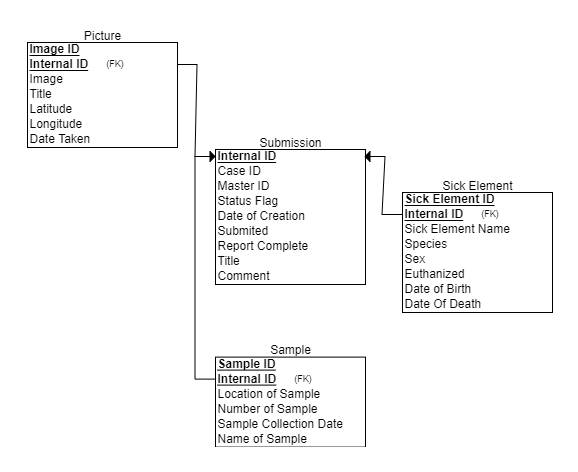
\includegraphics[scale=.45]{SqliteAlpha.png}
}
\caption{SqLite Alpha Phase}
\end{figure}

\begin{figure}
\begin{itemize}
    \item KEY:
    \begin{itemize}
        \item Red: Both MySql and SqLite need this table added.
        \item Blue: Only MySql need this table added.
        \item Green: Both MySql and SqLite have this table implemented. 
    \end{itemize}
\end{itemize}


 \centering{
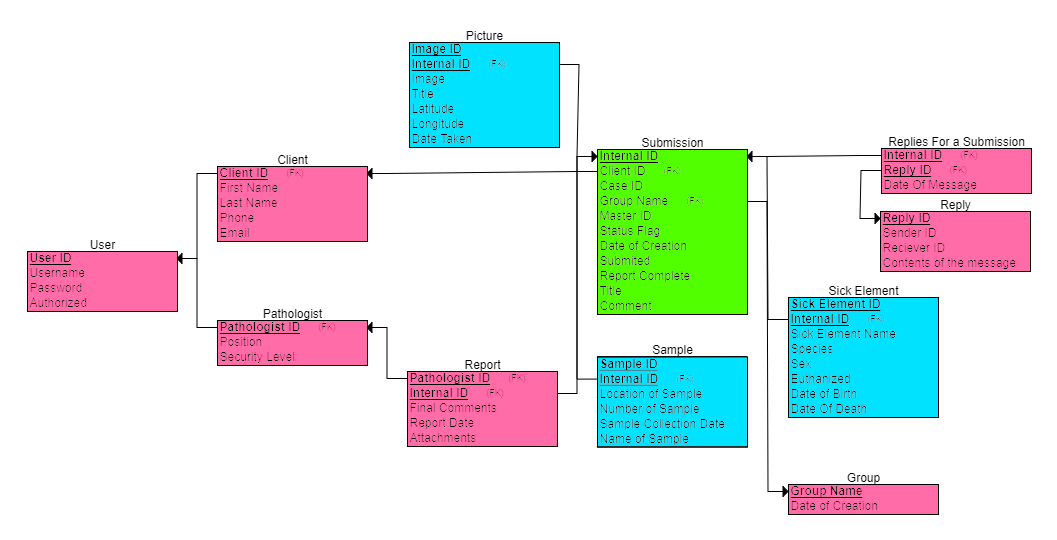
\includegraphics[scale=.45]{FinalDB.png}
}
\caption{Future Plans for Databases}



\end{figure}


\begin{center}
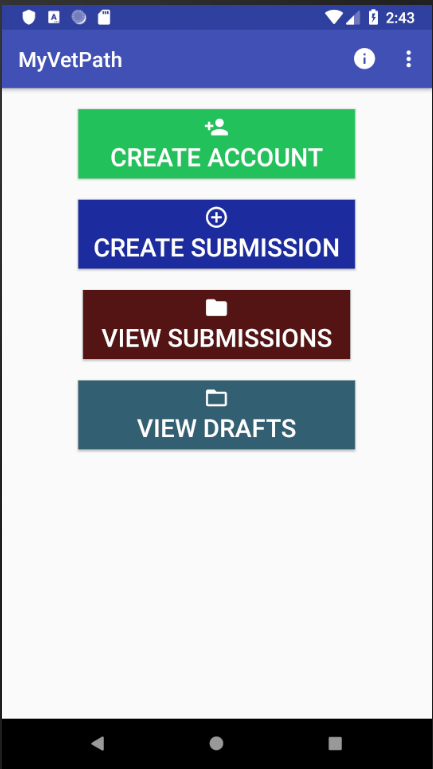
\includegraphics[height=8cm]{home.png}
\end{center}
\captionof{figure}{Home Screen}

\begin{center}
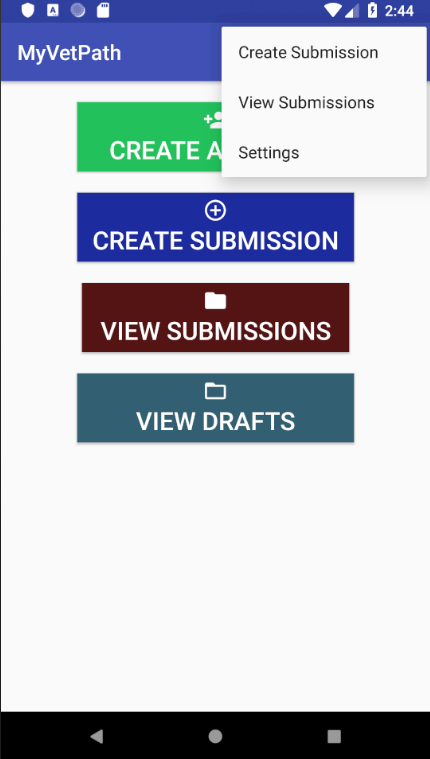
\includegraphics[height=8cm]{toolbar.png}
\end{center}
\captionof{figure}{Toolbar}

\begin{center}
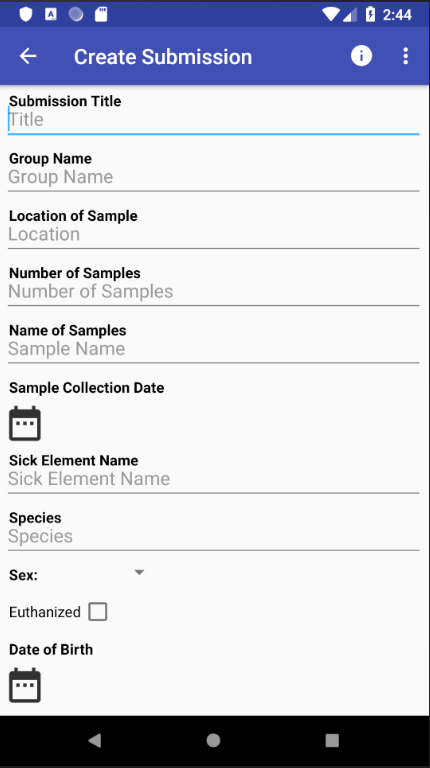
\includegraphics[height=8cm]{create_subs.png}
\end{center}
\captionof{figure}{Create Submissions Screen}

\begin{center}
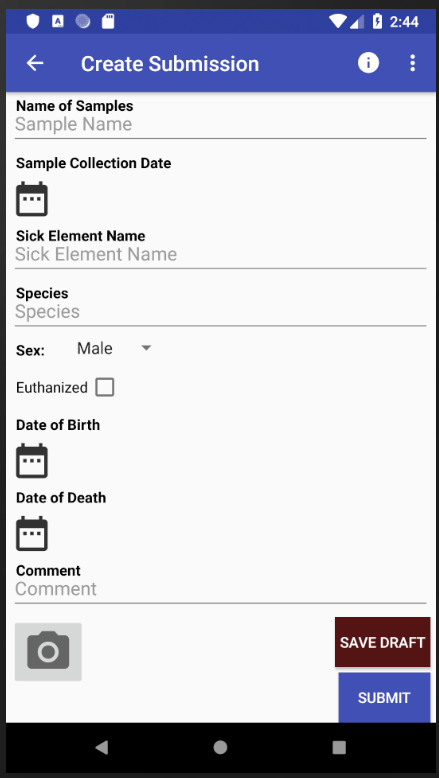
\includegraphics[height=8cm]{create_subs_pt2.png}
\end{center}
\captionof{figure}{Create Submissions Screen Part 2)}


\begin{center}
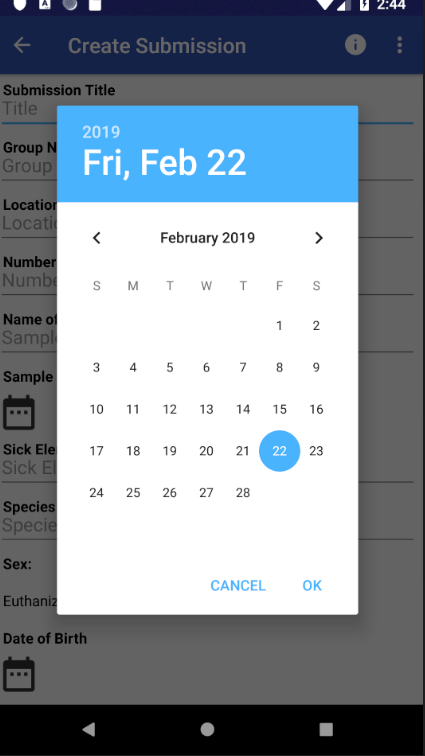
\includegraphics[height=8cm]{datePickerFragment.png}
\end{center}
\captionof{figure}{Date Picker}

\begin{center}
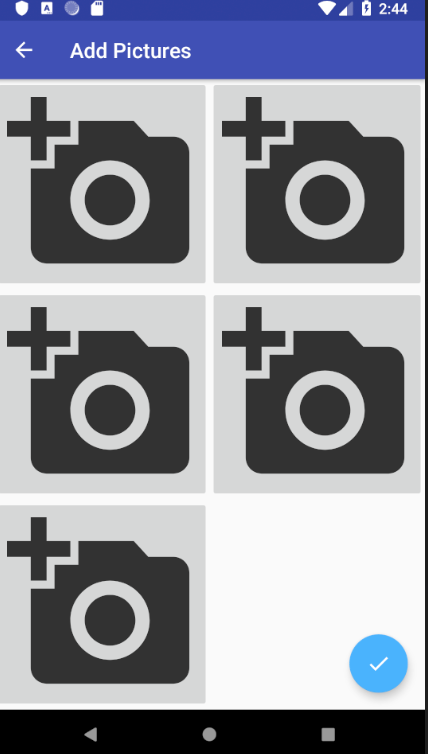
\includegraphics[height=8cm]{add_pictures.png}
\end{center}
\captionof{figure}{Add Pictures Screen}

\begin{center}
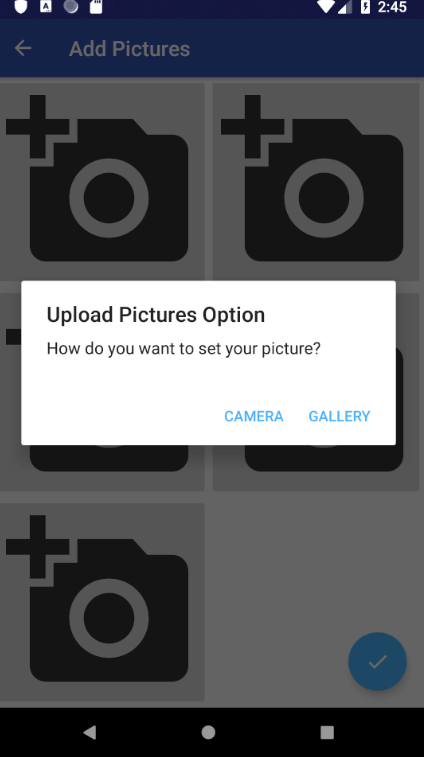
\includegraphics[height=8cm]{add_pictures_choice.png}
\end{center}
\captionof{figure}{Add Pictures Prompt}


\begin{center}
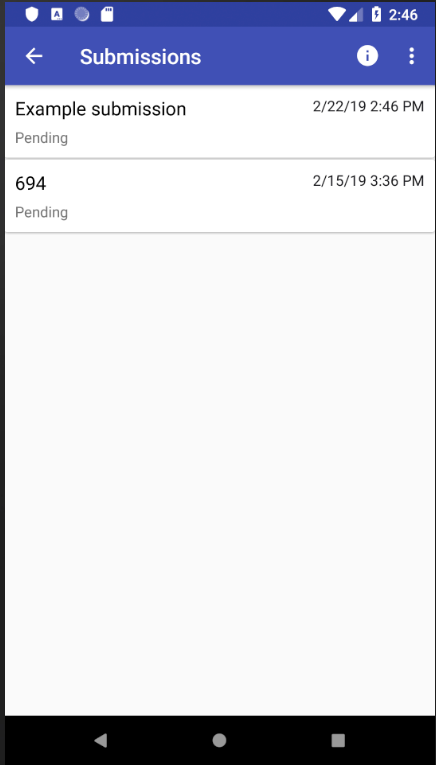
\includegraphics[height=8cm]{Viewsubmissions.png}
\end{center}
\captionof{figure}{View Submissions Screen}

\begin{center}
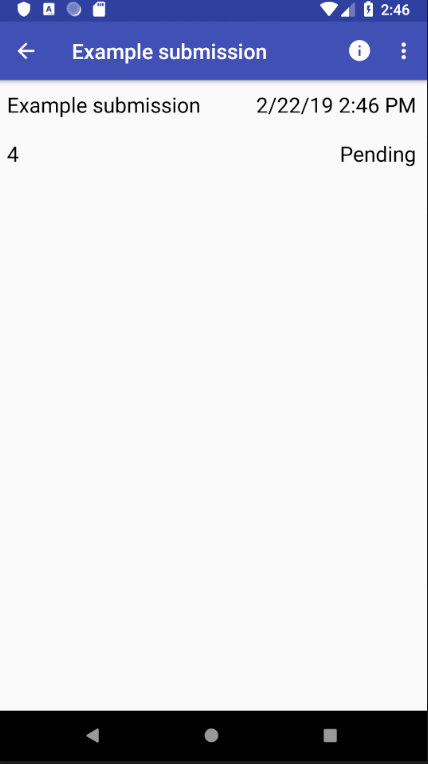
\includegraphics[height=8cm]{detail_view_submissions.png}
\end{center}
\captionof{figure}{Detailed View Submissions Screen}

\begin{center}
    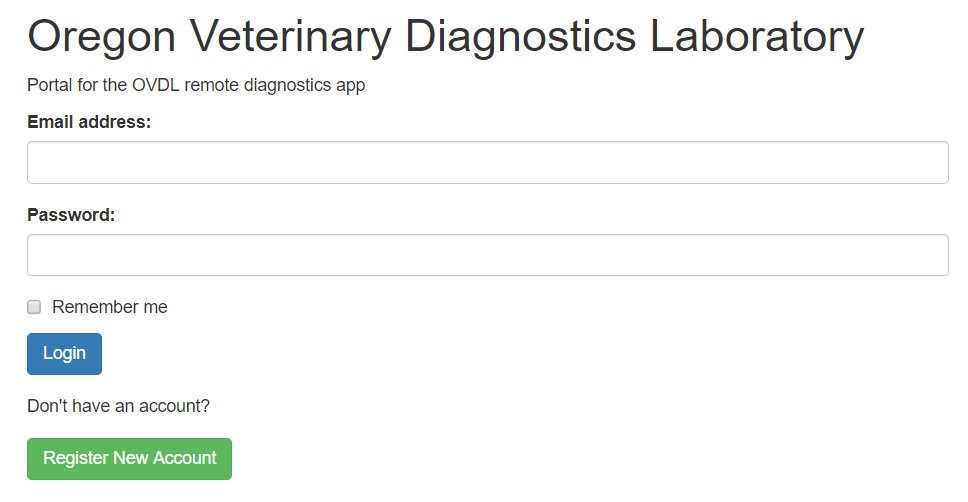
\includegraphics[height=6cm]{login_web.png}
\end{center}
\captionof{figure}{Website Login Screen}

\begin{center}
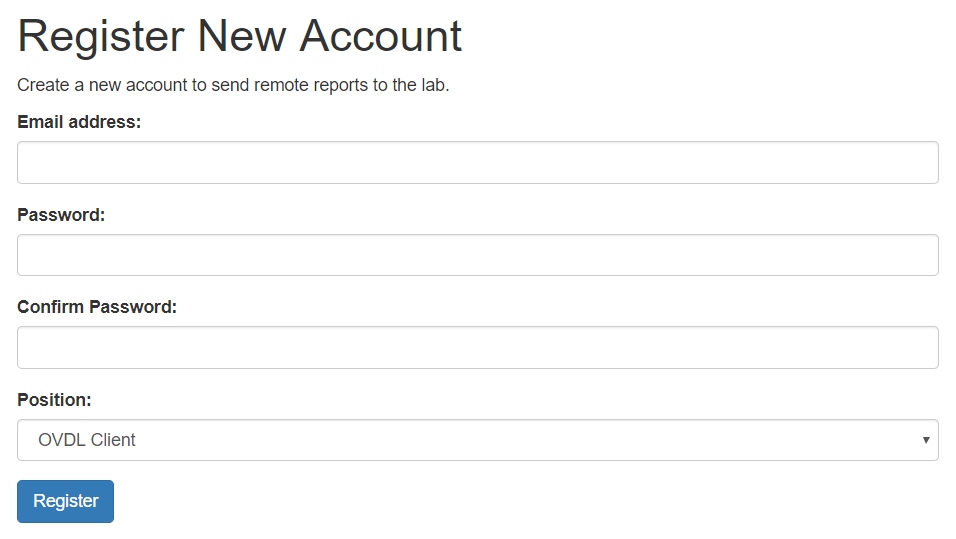
\includegraphics[height=6cm]{register_web.png}
\end{center}
\captionof{figure}{Website Registration Screen}



\end{document}